\documentclass[a4paper, halfparskip, onecolumn, abstracton, final, figurecaptionabove]{scrartcl}

\usepackage{natbib, url, listings, covington}
\usepackage[flushleft,alwaysadjust]{paralist}
\usepackage[]{epsfig}
\usepackage[]{natbib}
\bibpunct[,]{(}{)}{;}{a}{}{,}
\bibliographystyle{LandPModMod}

%\usepackage{ngerman}
%\usepackage{tipa}
\usepackage{graphics,latexsym}
%\usepackage{longtable}
%\usepackage{rotating}

\usepackage[inner=3cm,outer=3cm,top=2.5cm,bottom=2.5cm]{geometry}
%\setlength\parskip{\smallskipamount} \setlength\parindent{0pt}

\newcommand{\noun}[1]{\textsc{#1}}

%\renewcommand{\section}{\normalfont}
%\large\sffamily\bfseries}

%\\[5ex]

% doppelzeilig -- fuer 1 1/2 den Wert 1.3 nehmen!
%\linespread{1.3}

\usepackage{setspace}
\doublespacing

\begin{document}
%\begin{titlepage}
\titlehead{}
\subject{\normalsize Abstract of a Paper for \emph{Advances in FDG} based on a Poster presented at ICFG12}
%\title{Generating linguistic expressions from underlying clause structures\\[0.2cm]\Large A modular implementation}
\title{\Large Computational Representation of Underlying Structures and Lexical Entries using Domain-Specific Languages}
%\title{Formal Notation in Linguistic Description \\using Domain-Specific Languages}
%\title{Formal Linguistic Notation using Domain-Specific Languages}
%\title{\LARGE A Modular Functional Grammar Language Generator}
\author{Fabian Steeg, Christoph Benden, Paul O. Samuelsdorff \\ \small Linguistic Information Processing, Department of Linguistics, University of Cologne}

\maketitle

%\abstract{We describe a modular system for generating sentences using domain-specific languages for the representation of underlying structures and lexical entries. The system is implemented using Prolog, Java and ANTLR and can be used in the context of a larger NLP system for language generation or as a tool for formal notation in linguistic description. }

\marginline{}

%\thispagestyle{empty}


%\tableofcontents
%\listoffigures

%\end{titlepage}

%\maketitle 
%\thispagestyle{empty}

%\newpage

%\listoftables

%\pagenumbering{arabic}
\section{Motivation and Overview}
%\footnote{Source code, documentation and infrastructure for collaborative work, like a forum and a Subversion repository, is available under \textless http://fgram.sourceforge.net/\textgreater .}
This abstract describes a modular implementation of a system for generating sentences, using domain-specific languages (DSL; see section \ref{dsls}) for the formal representation of underlying structures and lexical entries. The DSL implemented for underlying structures is based on representations in Functional Grammar (FG; \citealt{Dik1997a}). Starting with a fully specified underlying structure instead of selecting lexical entries as the first step corresponds to the shift of Functional Discourse Grammar (FDG) to a top-down organization \citep{HengeveldAndMackenzie2006}. Through its modular architecture the system can be extended for formal representations in FDG. The idea of creating a computational implementation of FG and FDG mechanisms, to ``build a model of the natural language user'' \citep[1]{Dik1997a} is central to these frameworks and a valuable evaluation tool for linguistic theories in general, since ``linguistics may learn from being applied'' \citep[4]{Bakker1994}. Therefore our implementation can be used to evaluate and improve FDG with respect to theoretical issues in language generation. FDG demands ``formal rigor'' \citep[668]{HengeveldAndMackenzie2006} and accordingly should be tested formally. Our implementation can therefore be used to evaluate and improve representational aspects of FDG. The expression rules and the lexicon are based on a revised and extended version of the implementation described in \cite{Samuelsdorff1989}. By means of its modular architecture the program could act as the language generation component in a larger natural language processing (NLP) system or as a tool for formal notation in linguistic description.

\section{System Architecture}

\begin{figure}
\begin{center}
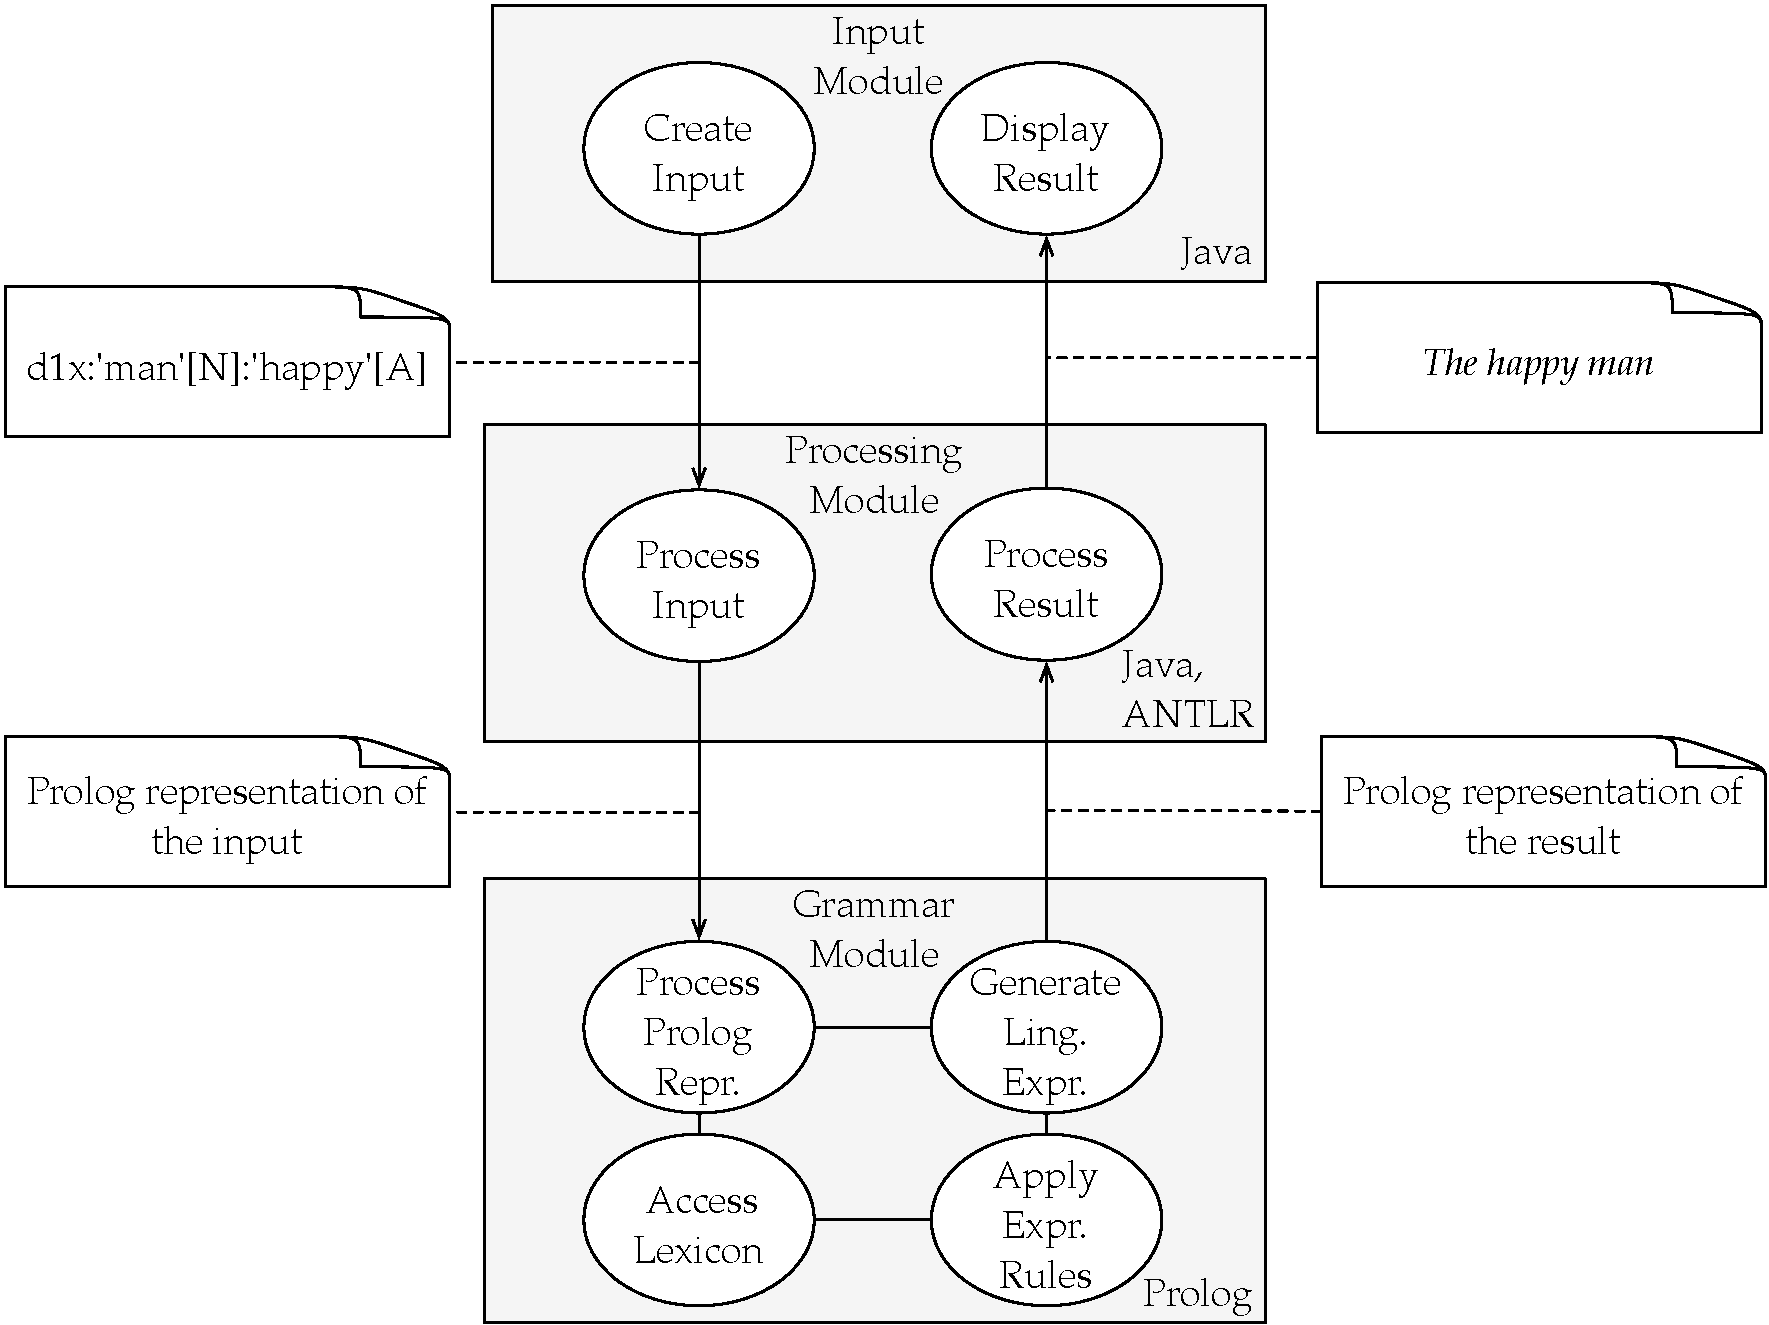
\epsfig{file=architecture.pdf, width=15cm}
\end{center}
\caption{System Architecture} \label{sysflow}
\end{figure}

%The system consists of three modules. The graphical user interface (GUI) assists the user in entering a valid formal represenation (\emph{input module}). When a valid formal representation is entered, the input is converted into a representation of the input in Prolog (\emph{processing module}). This representation is then used by the \emph{grammar module} to generate the linguistic expression. The result is passed back by the \emph{processing module} to the \emph{input module} to display the linguistic expression generated from the original input entered by the user. For an overview of the described interaction of the system modules see figure \ref{sysflow}. The system architecture can be characterized as a Model-View-Controller (MVC) or three-tier architecture. 

%\footnote{For calling Prolog from Java we use Interprolog (http://www.declarativa.com/interprolog/). The Prolog implementation we use is SWI-Prolog (http://www.swi-prolog.org/).}

The system consists of individual, exchangeable modules for creating an underlying structure, processing that input and generating a linguistic expression from the input (see Fig. \ref{sysflow}). In the \emph{input module} an underlying structure is created, edited and evaluated. Upon evaluation the input is sent to the \emph{processing module}, which communicates with the \emph{grammar module}. When the generation is done, the graphical user interface (GUI) displays either the result of the evaluation, namely the linguistic expression generated from the input, or an error message. The system architecture can be characterized as a Model-View-Controller (MVC) or three-tier architecture. Such a modular approach has two main advantages: First, modules can be exchanged; for instance the \emph{input module} is implemented both as a desktop application and as a web-based user interface with the actual processing happening on a server (implemented using Java Server Pages on a Tomcat servlet container). Second, by using a defined input format, our system can be combined with other NLP components and be reused in new contexts.

\section{Domain-Specific Languages}\label{dsls}
%\footnote{An example of combining Java and Prolog in a similar fashion is described in \cite{Macks2002}.}
The usage of languages which are tailored for a specific domain (domain-specific languages, DSL) has a long tradition in computing and has been acknowledged as a best practice in recent years (cf. \citealt[Ch. 12]{HuntAndThomas1999} and \citealt{Parr2007}). Our system uses Java as a general-purpose language, Prolog as a DSL for lexical entries and expression rules, and a self-defined DSL for describing underlying structures, implemented using ANTLR, a tool for defining and processing domain-specific languages \citep{Parr2007}. While e.g. in the domain of banking a DSL might describe credit rules, a linguist working with a model like FDG uses a DSL for linguistic description, e.g. for formal notation of underlying structures. With ANTLR, the form of the DSL is defined in EBNF notation, based on which a Java parser that can process the DSL is automatically generated, allowing for interaction with the abundant supply of libraries available in Java.


\begin{figure}
\begin{center}
\mbox{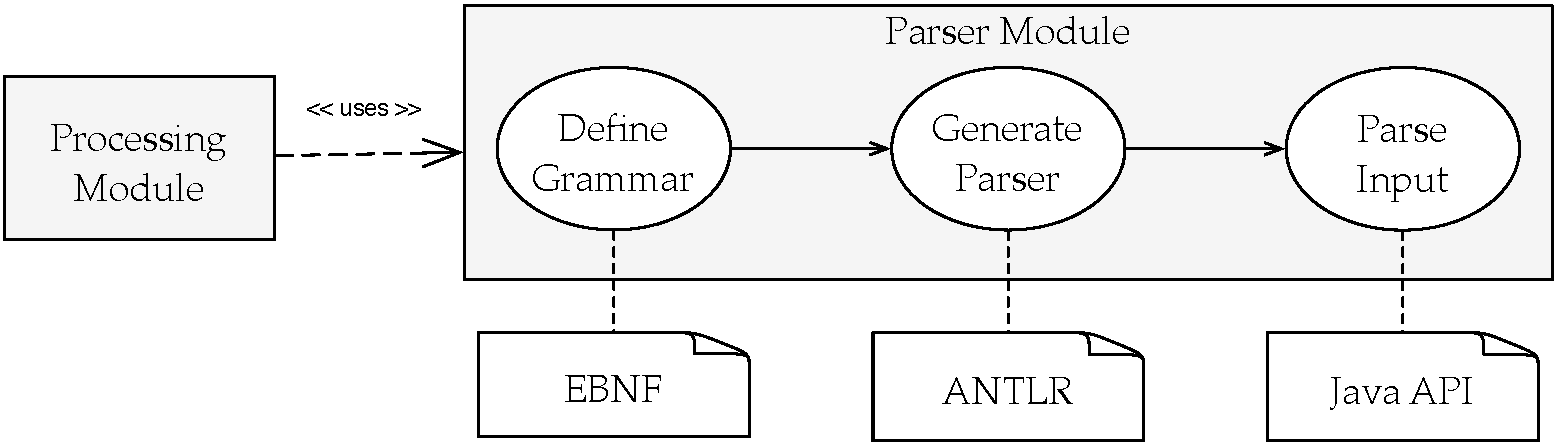
\epsfig{file=parser.pdf, width=15cm}}
\end{center}
\captionabove{Parser overview} \label{antlr-rl}
\end{figure}


%Java is a widespread multi-purpose programming language with abundant supply of libraries.

%(Fig. \ref{antlr-def} shows a part of the ANTLR grammar definition file)

%Just like programming languages, underlying structures in models like FG and FDG are formal languages and can therefore be seen as domain-specific languages for linguistic description.

%The reason for using Java for the user interface and processing of the input, ANTLR for the definition of the input format grammar and Prolog for the expression rules and the lexicon is based on the goal of using implementation languages well suited for a particular task.

%The generated parser for the language is a Java class; 

\section{Underlying Structures}

The \emph{processing module's} input format is a representation of the linguistic expression to be generated; its form is based on the representation of underlying structures given in \cite{Dik1997a}. The \emph{processing module} parses the input entered by the user (or potentially coming from a different source) and creates an internal representation (see Fig. \ref{uml-tree}) which is then converted into the output format of the \emph{processing module}, a Prolog representation of the input, which is used by the \emph{grammar module}.

\begin{figure}
    \begin{center}

% LEXICON
\begin{verbatim}
(Past e:
    (d1x:'man'[N]:
        (Past Pf e:'give'[V]
            (d1x:'mary'[N])Ag  
            (dmx:'book'[N]:'old'[A])Go
            (x:'man'[N])RecSubj
        )
    )
    (d1x:'john'[N])0
)
\end{verbatim}


\captionabove{A nested underlying structure based on \cite{Dik1997a}, which is parsable by the generated ANTLR parser (represents \emph{John is the man who was given the book by Mary})}\label{antlr-input}

    \end{center}
    \end{figure}
    
    \begin{figure}
     \begin{center}
  
\begin{verbatim}
(p1: 
    [ 
        (Past e1: 
            [
                (f1:tek(
                    (x1:im(x1))Ag
                    (x2:naif(x2))Inst
                )(f1))
                (f2:kot(
                    (x1:im(x1))Ag
                    (x3:mi(x3))Pat
                )(f2))
            ](e1)
        )
    ](p1)
)
\end{verbatim}

%\end{examples}

\captionabove{Underlying structure on the RL in FDG (Jamaican Creole: \emph{Im tek naif kot mi}, 'He cut me with a knife')}\label{fdg-rl}  
\end{center}
\end{figure}

Figures \ref{antlr-input} and \ref{fdg-rl} show the structural similarity of underlying structures in FG and FDG; both representations are nested parentheses, which can also be represented as trees (cf. Fig. \ref{uml-tree}). Since these representations can be described and processed with the same mechanisms, and representations on all levels of FDG have a common scheme \citep[671]{HengeveldAndMackenzie2006}, support for FDG representations is easy to add by supplying ANTLR definitions for representations on the individual levels in FDG, like the Interpersonal Level (IL) and the Representational Level (RL). Such an implementation will be described in our paper and will provide a validator for the formal structure of IL and RL representations. With grammar files for the IL and the RL implemented and having an internal representation of the input, alternative processing is possible too, like output of typeset representations of the underlying structures with and without indentation, e.g. with output looking like the underlying structure in Fig. \ref{fdg-rl}.

\begin{figure}

\begin{verbatim}
move
  :  '(' 'M' INDEX ':' '['
        act+
  ']' '(' 'M' INDEX ')' ( ':' WORD '(' 'M' INDEX ')' )* ')' ;
			
act
  :  '(' 'A' INDEX ':' '['
        ( speech_occurence
        | speaker
        | addressee
        | communicated_content
        )*
  ']' '(' 'A' INDEX ')' ( ':' WORD '(' 'A' INDEX ')' )* ')' ;
\end{verbatim}

\captionabove{ANTLR grammar definitions for the Move and the Act} \label{antlr-def1}
\end{figure}

\begin{figure}
\begin{center}
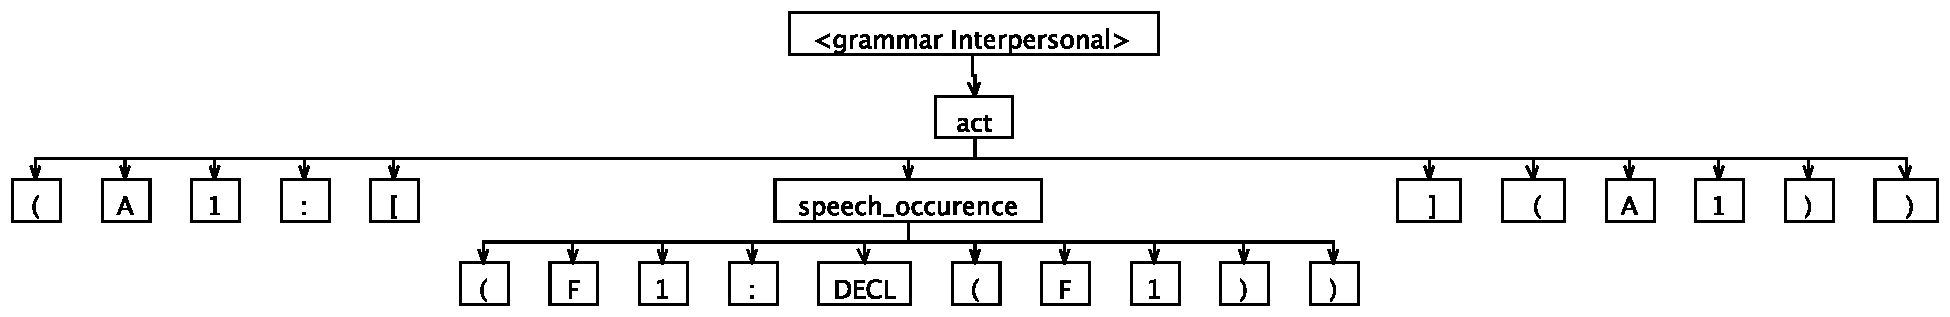
\epsfig{file=act-tree.pdf, width=15cm}
\end{center}
\captionabove{Parse tree for the act '(A1:[(F1:DECL(F1))](A1))'} \label{antlr-il}
\end{figure}

\begin{figure}

\begin{verbatim}
propositional_content
  :  '(' OPERATOR 'p' INDEX ':' '[' 
          state_of_affair+ 
     ']' '(' 'p' INDEX ')' (':' WORD '(' 'p' INDEX ')')* ')' FUNCTION? ;

state_of_affair 	
  :  '(' OPERATOR 'e' INDEX ':' '[' 
        ( property 
        | individual 
        | location 
        | time
     )* 
']' '(' 'e' INDEX ')' (':' WORD '(' 'e' INDEX ')')* ')' FUNCTION?	;
\end{verbatim}

\captionabove{ANTLR grammar definitions for the Proposition and a State-of-Affair} \label{antlr-def2}
\end{figure}

\begin{figure}
\begin{center}
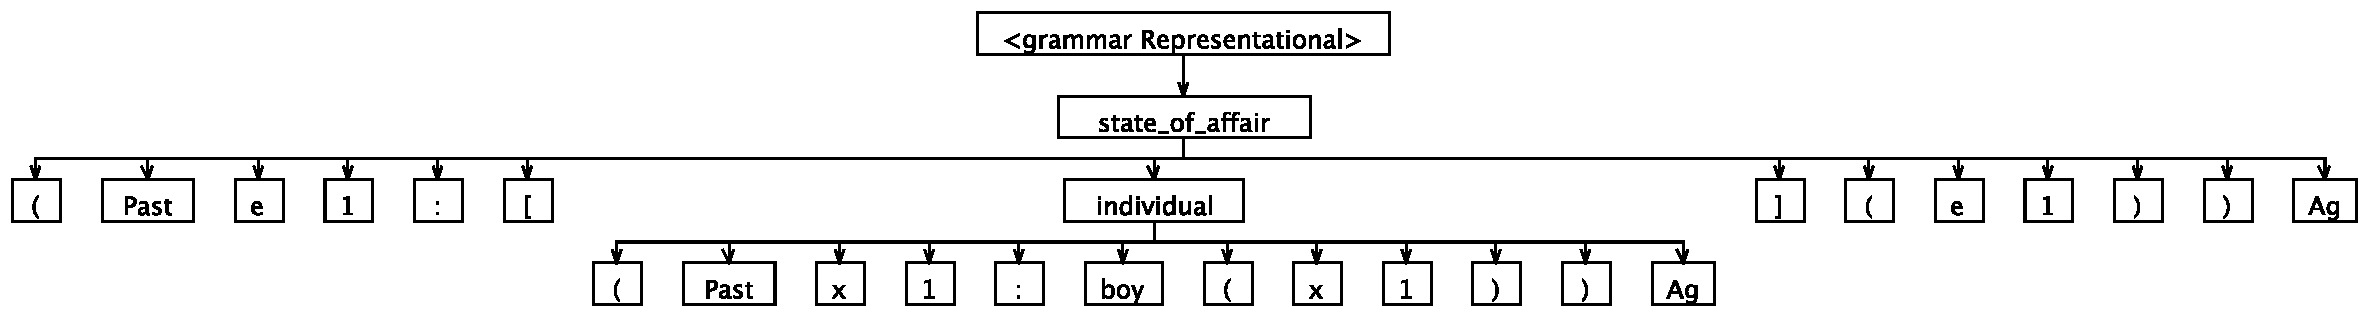
\epsfig{file=soc-tree.pdf, width=15cm}
\end{center}
\captionabove{Parse tree for the state of affair '(Past e1: [(Past x1:boy(x1))Ag](e1))Ag'} \label{antlr-rl}
\end{figure}

%The structure of formal representations in FG and FDG is very similar, see Fig. \ref{antlr-input} for an underlying structure in FG and Fig. \ref{fdg-il} and \ref{fdg-rl} for underlying structures in FDG (Jamaican Creole: \emph{Im tek naif kot mi}, 'He cut me with a knife'). All these structures are nested parenthesis expressions, which can also be represented as trees (cf. Fig. \ref{ucs} and \ref{uml-tree}). Since these structures can be described and processed with the same mechanisms, and underlying structures in FDG all conform to a common structure \citep[671]{HengeveldAndMackenzie2006}, support for FDG representations on the input level is easy to add by supplying ANTLR  grammar files for the different levels like the Interpersonal Level (IL) and the Representational Level (RL). Such an implementation is planned and will be described in our paper; this would effectively provide a validator for the formal structure of IL and RL representations. With grammar files for IL and RL implemented and having an internal representation of the input, alternative processing is possible too, like output of typeset representations of the structure with and without indentation, e.g. as given in Fig. \ref{fdg-il} and \ref{fdg-rl}.

%For representing underlying structures in a form as close to convention as possible, we define a DSL using ANTLR, a specialized grammar description language and parser generator \citep{Parr2007}.

%\begin{figure}
%  \begin{minipage}{0.48\textwidth}
%    \begin{center}

%\begin{footnotesize}
%\begin{verbatim}
%(Past Pf e:'give' [V]:
%    (dmx:'farmer' [N]:'old' [A])AgSubj
%    (imx:'duckling' [N]:'soft' [A])GoObj
%    (dmx:'woman' [N]:'young' [A])Rec
%)
%\end{verbatim}
%\end{footnotesize}
%%\normalsize
%\caption[Sample input]{Input format: the DSL for underlying structures (generates  \emph{The old farmers had given soft ducklings to the young women})}
%\label{ucs}

%
%    \end{center}
%  \end{minipage}% Dies Prozent ist wichtig! (kein horiz. Abst. zw. minipages)
%  \begin{minipage}{0.04\textwidth}
%     \hfill % Damit die getrennte Beschriftung auch Abstand hat
%  \end{minipage}%
%  \begin{minipage}{0.48\textwidth}
%    \begin{center}
%      \mbox{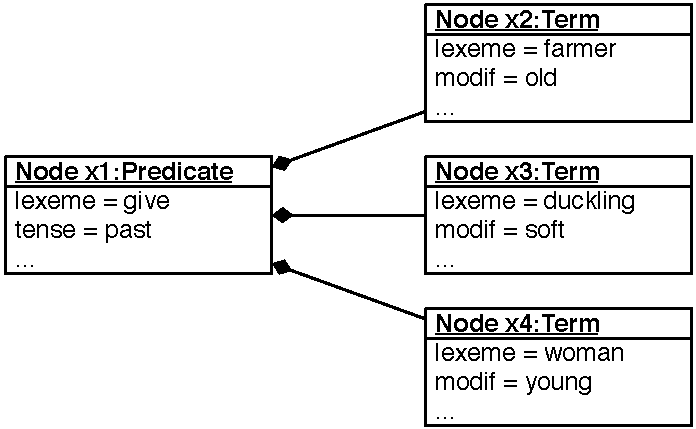
\epsfig{file=objects.pdf, height=3cm}}
%\caption{Internal representation of the input: a tree of Java objects (in UML notation)}
%\label{uml-tree}
%    \end{center}
%  \end{minipage}
%\end{figure}

\section{Lexical Entries}

In the \emph{grammar module} the Prolog representation of the input generated by the \emph{processing module} is used to generate a linguistic expression. Prolog was developed as a programming language for linguists and therefore offers convenient notation and processing mechanisms, e.g. lexical entries can be stored directly as Prolog facts (see Fig. \ref{prolog-2}). Prolog also has a particular strong standing as an implementation language for FG (e.g. \citealt{Samuelsdorff1989,Dik1992}). By restricting the usage of Prolog to lexical entries and expression rules and combining it with other languages, instead of using it as a general-purpose programming language for the entire program, we use Prolog as a DSL in its original domain. The expression rules and the lexicon are based on a revised and extended version of the implementation described in \cite{Samuelsdorff1989}. To make the implementation work as a module in the described system, the user dialog of the  original version (in which the underlying structure is built step by step) was replaced by an immediate processing of the entire input representing the linguistic expression to be generated. The user dialog is therefore replaced by the formal representation, which is created in the \emph{input module} and converted into a Prolog representation by the \emph{processing module}. This resembles the shift to a top-down organization in FDG \citep{HengeveldAndMackenzie2006}, where the conceptualization is the first step, not the selection of lexical elements, as it was in FG and in our original implementation.

%In the original implementation the underlying structure is subsequently built via a user dialog, during which the expression to be generated is specified step by step.

\begin{figure}
    \begin{center}
%\begin{footnotesize}
%\begin{tabbing}
% (M$_1$:\= [ (A$_1$: [ (F$_1$:DECL) (P$_1$) (P$_2$)\\
%	 \>(C$_1$:[\=\\
%	 	\>\>[T$_1$:\emph{tek}(\=\\
%		\>\>\>	(R$_1$:\emph{im})\\
%		\>\>\>	(R$_2$:\emph{naif})\\
%		\>\>)]\\
%		\>\>[T$_2$:\emph{kot}(\\
%		\>\>\>	(R$_1$)\\
%		\>\>\>	(R$_3$:\emph{mi})\\
%		\>\>)]\\
%	\>]) \\
%	]) ])
%\end{tabbing}
%\end{footnotesize}
%\captionabove{Underlying structure on the IL (Jamaican Creole: \emph{Im tek naif kot mi}, 'He cut me with a knife')} \label{fdg-il}

   \mbox{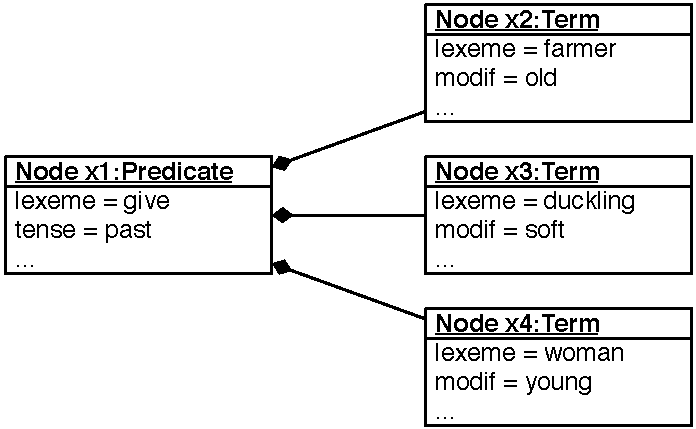
\epsfig{file=objects.pdf, height=5cm}}
\caption{Internal representation of an underlying structure: a tree of Java objects (in UML notation)}
%for \emph{The old farmers had given soft ducklings to the young women}
\label{uml-tree}
 
    \end{center}
    \end{figure}
    
    \begin{figure}
      \begin{center}

 \begin{verbatim}
verb(
    give, 
    action, 
    [gave, given], 
    [
        [agent, animate, X1], 
        [goal, any, X2],
        [recipient, animate, X3]
     ], 
     Sat
).
\end{verbatim}

\captionabove{Ditransitive verb as a Prolog fact in the lexicon} \label{prolog-2}

    \end{center}
\end{figure}

  
 
%\begin{figure}
%  \begin{minipage}{0.48\textwidth}
%    \begin{center}
%\begin{footnotesize}
%% LEXICON
%\begin{verbatim}
%verb(
%    believe, 
%    state, 
%    [regular, regular], 
%    [
%        [experiencer, human, X1], 
%        [goal, proposition, X2]
%        
%    ], 
%    Sat
%).
%\end{verbatim}
%\end{footnotesize}

%\captionabove{Transitive verb as a Prolog fact in the lexicon} \label{prolog-1}

%    \end{center}
%  \end{minipage}% Dies Prozent ist wichtig! (kein horiz. Abst. zw. minipages)
%  \begin{minipage}{0.04\textwidth}
%     \hfill % Damit die getrennte Beschriftung auch Abstand hat
%  \end{minipage}%
%  \begin{minipage}{0.48\textwidth}
%    \begin{center}
%    
% \begin{footnotesize}
% \begin{verbatim}
%verb(
%    give, 
%    action, 
%    [gave, given], 
%    [
%        [agent, animate, X1], 
%        [goal, any, X2],
%        [recipient, animate, X3]
%     ], 
%     Sat
%).
%\end{verbatim}
%\end{footnotesize}
%\captionabove{Ditransitive verb as a Prolog fact in the lexicon} \label{prolog-2}
%    \end{center}
%  \end{minipage}
%  \end{figure}

%[...]
%noun(axe,instrument,[regular,neuter],[[argument,instrument,X]],Sat).
%noun(book,readable,[regular,neuter],[[argument,readable,X]],Sat). 
%[...]
%adj(big,size,[[],big],[[argument,any,X]],Sat).
%adj(eager,quality,[[],eager],[[first_argument,animate,X1],[second_argument,infinitive,X2]],Sat).
%[...]


% GRAMMATICON
%be([[was,past,sing], [were,past,plural], [is,present,sing],[are,present,plural]]).
%have([[had,past,N],[has,present,sing],[have,present,plural]]).
%do([[did,past,N],[does,present,sing],[do,present,plural]]).
%determiner([["the",def,N,G],["a",indef,sing,G],["every",total,sing,G],[...]
%pronouns([[he,pers,masc,sing,subj],[him,pers,masc,sing,ob],[she,pers,fem,sing,subj],[...]

\begin{figure}
\begin{center}
\fbox{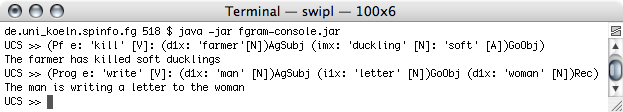
\epsfig{file=screen1.png, width=15cm}}
\end{center}
\captionabove{Screenshot of the console-based implementation} \label{antlr-rl}
\end{figure}


\begin{figure}
\begin{center}
\fbox{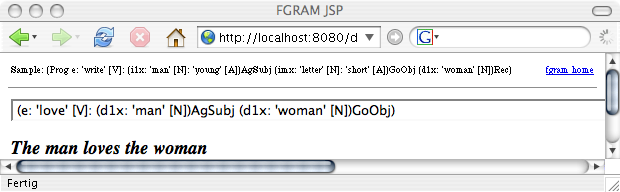
\epsfig{file=screen2.png, width=15cm}}
\end{center}
\captionabove{Screenshot of the Web-based implementation} \label{antlr-rl}
\end{figure}


\section{Conclusion}
\normalsize
We describe a modular implementation of a language generation system, representing underlying structures and lexical entries using domain-specific languages. The system makes use of an input format based on \cite{Dik1997a} and consists of modules implemented in Java, Prolog and ANTLR, making it easy to extend for FDG representations. The system can be used to evaluate and improve FDG with respect to theoretical and representational issues; by means of its modular architecture it could act as the language generation component in a larger NLP system or as a tool for formal notation in linguistic description.

%\newpage
%\thispagestyle{empty}
%\enlargethispage{1cm}
\bibliography{fsteeg}

%\newpage
%\section*{References}

%\begin{description}

%\item [\textmd{\noun{Bakker}}\textmd{,}]Dik. {}1994 ``Formal and Computational Aspects of Functional Grammar and Language Typology''. Amsterdam: IFOTT.

%\item [\textmd{\noun{Dik}}\textmd{,}]Simon C. 1992 {}``Functional Grammar in Prolog; an integrated implementation for English, French and Dutch''. Berlin, New York: Mouton de Gruyter. 

%\item [\textmd{\noun{Dik}}\textmd{,}]Simon C. {}\& Kees \noun{Hengeveld}. 1997 ``The Theory of Functional Grammar, Part 1: The Structure of the Clause''. Berlin, New York: Mouton de Gruyter. 

%\item [\textmd{\noun{Macks}}\textmd{,}]Aaron. 2002 {}``Parsing Akkadian Verbs with Prolog''. 27. November 2005 \textless www.cs.um.edu.mt/\textasciitilde mros/WSL/papers/macks.pdf\ %\textgreater

%\item [\textmd{\noun{Samuelsdorff}}\textmd{,}]Paul-Otto. 1989 {}``Simulation of a
%Functional Grammar in Prolog'' In: \noun{Connolly}, John H. \& Simon C.
%\noun{Dik} (eds.) \emph{Functional Grammar and the Computer.} 29-44\emph{.} Utrecht, Providence: Foris Publications.

%\item [\textmd{\noun{Samuelsdorff}}\textmd{,}]Paul-Otto. 1998 {}``Pronouns, Adpositions, ``Adverbs" and the Lexicon'' In: \noun{Olbertz}, Hella, Kees  \noun{Hengeveld} \& Jes\'us S\'anchez \noun{Garc\'ia} (eds.) \emph{The Structure of the Lexicon in Functional Grammar.} 267-278\emph{.} Amsterdam, Philadelphia: John Benjamins Publishing Company.
%\end{description}

\end{document}
